\chapter{Sensor Fusion}
Nei sistemi in cui \`e richiesta un'alta \emph{reliability} delle misure, l'informazione fornita dai singoli sensori non \`e sufficiente. In questi casi \`e raccomandato l'utilizzo di un insieme di sensori in contemporanea. \cite{sfarailway}
\section{Panoramica}
In generale, un algoritmo SFA viene utilizzato per stimare lo stato di un sistema dinamico in un ambiente caratterizzato da \emph{rumore}. \cite{kfbook}
\subsection{Sistemi Dinamici}
Un sistema dinamico \`e una modellazione matematica di un processo che evolve nel tempo, la cui evoluzione \`e descritta attraverso un sistema di equazioni differenziali o alle differenze, nel caso esso si evolva rispettivamente a tempo continuo o a tempo discreto.\\*
Sia $S$ l'insieme dei possibili stati che il sistema pu\`o assumere, e sia $m = |S|$ la dimensione dello spazio degli stati.\\*
Senza perdere in generalit\`a, si possono formalizzare questi due tipi di sistemi dinamici come:
$$
y'(t) = f(t,y(t)),\;t\ge 0\;\;\;\;(1)
$$
Con $y(0) \in \mathbb{R}^m$ condizione iniziale nota, e:
$$
y_{n+1} = f(n,y_n),\;n = 0,1,\dots\;\;\;\;(2)
$$
con al solito $y_0 \in \mathbb{R}^m$ condizione iniziale nota\;\cite{gigi}.\\*
Ricavare lo stato del sistema dinamico per un certo istante $t$, o $n$, equivale a risolvere le equazioni cui sopra e valutarne la traiettoria soluzione in $t$ o in $n$.\\*
Un semplice sistema dinamico \`e rappresentato da un punto materiale che si muove con una accelerazione costante $$\mathbf{a} = a\mathbf{k}$$ dove $\mathbf{k}$ \`e un qualunque versore della base canonica di $\mathbb{R}^3$.\\*
Supponendo che il punto si muova con velocit\`a iniziale $\mathbf{z'}(0) = v_0\mathbf{k}$ nota e inizi il moto da una coordinata $\mathbf z(0) = z_0\mathbf{k}$ nota, si ha:
$$
z''(t) = a\;\;\;\;(3)
$$
$$
z'(t) = \int{a dt} = a t + v_0
$$
$$
z(t) = \int(a t + v_0)dt = \frac{1}{2} at^2 +  v_0 t + z_0
$$
L'equazione $z(t)$ descrive completamente la traiettoria di moto del punto materiale, mentre $z'(t)$ descrive completamente la traiettoria della velocit\`a del punto durante il suo moto.
\subsubsection{Nota su sistemi dinamici continui e discreti}
Con l'introduzione del calcolatore come strumento di supporto al matematico applicato, sono stati sviluppati efficienti \emph{metodi numerici di approssimazione} che permettono di modellare un sistema dinamico continuo attraverso una sua \emph{controparte discreta}. Tale processo di discretizzazione \`e mirato alla definizione di un sistema dinamico che si comporti in maniera \emph{simile} al modello continuo che si intende studiare, dove per simile si intende che ne preservi il comportamento quantitativo e le caratteristiche asintotiche di stabilit\`a delle soluzioni.\\*
L'\emph{aritmetica finita} in cui lavora qualsiasi calcolatore rende indispensabile la discretizzazione dei modelli continui, ma d'altro lato l'esistenza dei metodi di approssimazione permette di restringere le discussioni che seguiranno considerando esclusivamente sistemi dinamici \emph{discreti}. \cite{gigi}
\subsection{Misure e Rumore}
Si consideri il sistema dinamico individuato dalla $(3)$.\\*
Le soluzioni esplicite della traiettoria del punto materiale sono valide, fatta assunzione di conoscere a priori il valore esatto di $a$, di $v_0$ e di $z_0$.\\*
Nella pratica, per misurare qualsiasi grandezza fisica \`e necessario uno strumento di misura, il quale produrr\`a delle misure affette da errori casuali.\\*
Si supponga di sostituire $a$ nell'equazione $z(t)$ con una sua perturbazione $\tilde{a} = a + \varepsilon$ dove $\varepsilon$ \`e una variazione casuale della misura data dal \emph{rumore} che caratterizza qualsiasi processo di misura. Si pu\'o supporre $Var(\varepsilon) = 0$ e considerare, ai fini di questa trattazione, $\varepsilon$ come un valore costante; in realt\`a $\varepsilon$ \`e una variable casuale a varianza generalmente non nulla. Si suppongano inoltre $v_0 = z_0 = 0$ per comodit\`a di calcolo:
$$
z(t) = \frac{1}{2} \tilde{a} t^2 = \frac{1}{2}(a + \varepsilon) t^2 = \frac{1}{2} \left(at^2 + \varepsilon t^2\right)
$$
Si nota immediatamente che la variazione della misura $z(t)$ data da $\varepsilon$ aumenta con il quadrato del tempo.\\*
\begin{figure}[h]
	\centering
	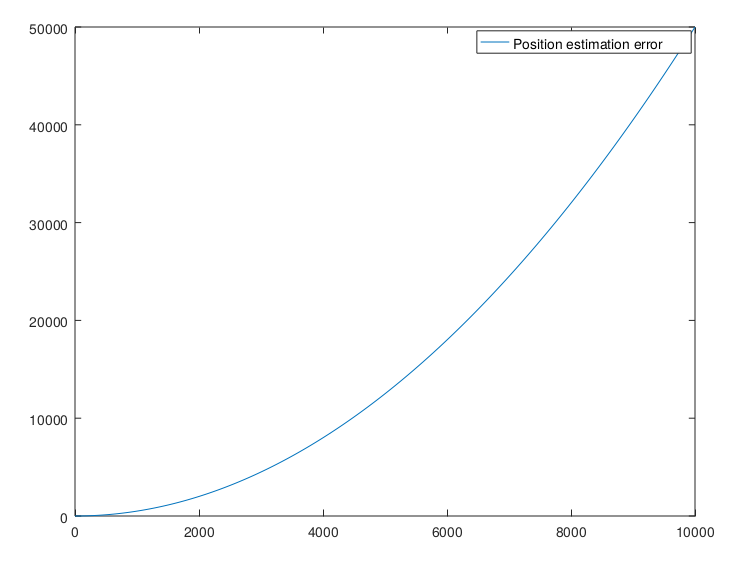
\includegraphics[scale=0.5]{img/errormeas}
	\caption{Grafico dell' errore di stima della posizione con $a = 10^0, \varepsilon = 10^{-3}$}
	\label{fig:errormeas}
\end{figure}\newpage
Il moto di un punto materiale soggetto a un' accelerazione nota, \`e una tipologia di sistema dinamico caratterizzato da assenza di \emph{rumore di processo}: fatta assunzione di conoscere esattamente il valore di $a$, la doppia integrazione di $(3)$ rispetto al tempo fornisce una descrizione esatta e deterministica della dinamica del sistema: la traiettoria sar\`a \emph{esattamente} quella individuata dalla soluzione.\\*
Alcuni processi tuttavia evolvono in parte stocasticamente per loro natura, e questa natura stocastica insita nel processo viene chiamata \emph{rumore di processo}. \cite{kfbook}\\*
Si consideri ad esempio il caso in cui la traiettoria di moto del punto materiale descritta dalle soluzioni della $(3)$ venga disturbata dall'azione di forze casuali, quali ad esempio improvvise raffiche di vento.\\*
La conclusione \`e che in molte applicazioni reali, non solamente le misurazioni sono affette da rumore, ma anche il processo evolutivo stesso pu\`o essere affetto da rumore stocastico intrinseco. La conseguenza \`e che la forma esplicita delle equazioni $(1)$ e $(2)$ contiene un termine casuale individuato da una variabile aleatoria.\\*
Uno schema di un processo caratterizzato da \emph{rumore} \`e mostrato in figura \ref{fig:mimo1}.
\begin{figure}[h]
	\centering
	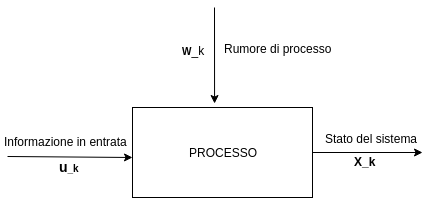
\includegraphics{img/mimo1}
	\caption{Processo caratterizzato da \emph{rumore}}
	\label{fig:mimo1}
\end{figure}
\section{I Filtri di Kalman}
Un Filtro di Kalman, o in inglese \emph{Kalman Filter} (KF), \`e uno \emph{stimatore} dello stato di un sistema dinamico caratterizzato da rumore. L'algoritmo individuato dalla formulazione matematica di un KF pu\`o essere usato come SFA.
\subsection{Premesse statistiche}
Un insieme di $N$ sorgenti di misurazioni viene modellato come un insieme di $N$ variabili casuali.\\*
Siano $X_1,\dots,X_N$ $N$ variabili casuali a valori in un insieme finito non vuoto $\mathbb{X}$, e sia $X,Y$ una qualsiasi coppia presa tra le $N$ variabili casuali.\\*
Si chiama \emph{covarianza} di $X,Y$ la seguente quantit\`a:
$$
cov(X,Y) = \mathbb{E}\{[X-\mathbb{E}(X)][Y-\mathbb{E}(Y)]\}= \sigma_{XY}
$$
Si osservi che :
$$
cov(X,X) =  \mathbb{E}\{[X-\mathbb{E}(X)]X-\mathbb{E}(X)]\} = \mathbb{E}[X-\mathbb{E}(X)]^2 =\sigma^2_{X}
$$
Per un vettore di $N$ variabili aleatorie $X_1,\dots,X_N$, si definisce la matrice di \emph{varianza-covarianza}, o semplicemente matrice di \emph{covarianza}, la seguente matrice quadrata $N$\texttt{x}$N$:
$$
\Sigma = \left(\begin{matrix}
cov(X_1,X_1) && cov(X_1,X_2) && \dots && cov(X_1,X_N) \\
\vdots && \vdots && \vdots \\
cov(X_N,X_1) && cov(X_N, X_2) && \dots && cov(X_N,X_N)
\end{matrix}\right) 
$$
$$
 = \left(\begin{matrix}
\sigma^2_{X_1} && \sigma_{X_1,X_2} && \dots && \sigma_{X_1,X_N} \\
\vdots && \vdots && \vdots \\
\sigma_{X_N,X_1} && \sigma_{X_N, X_2} && \dots && \sigma^2_{X_N}
\end{matrix}\right)
$$
Un vettore di $N$ variabili casuali si dice congiuntamente \emph{gaussiano}, ossia distribuito secondo una distribuzione di probabilit\`a \emph{normale multivariata}, quando qualunque combinazione lineare non banale:
$$
Y = \sum_{i=1}^N \alpha_iX_i\;\;\alpha_i \in \mathbb{R}
$$
Ha distribuzione di probabilit\`a \emph{gaussiana}.
\subsection{Filtro di Kalman Lineare}
I KF sono comunemente basati su sistemi dinamici \emph{lineari} a tempo discreto.\\*
In questa sezione viene esposto il principio base del funzionamento di un semplice KF lineare, avente lo scopo di stimare lo stato di un sistema dinamico lineare in presenza di rumore di processo e rumore di misura.
\subsubsection{Definizione del problema}
Si consideri il seguente sistema dinamico lineare discreto:
$$
\begin{cases}
\mathbf x_k = A \mathbf x_{k-1} + B \mathbf u_k + \mathbf w_k \\
\mathbf y_k = C \mathbf x_k + \mathbf v_k
\end{cases}\;\;\;\;(4)
$$
In cui i vettori $\mathbf w_k$ e $\mathbf v_k$ rappresentano rispettivamente il rumore di processo e il rumore di misura. Si assumono \emph{congiuntamente gaussiani}, indipendenti e con matrici di covarianza $Q,R$ rispettivamente.\\*
Il vettore $\mathbf y_k$ rappresenta il vettore di misurazioni campionate all'istante $k$, mentre il vettore $\mathbf x_k$ rappresenta lo stato del sistema all'istante $k$.\\*
Le matrici $A$ e $B$ descrivono la dinamica del modello e si assumono note a priori, pena l'introduzione di errori sistematici, mentre la matrice $C$ descrive la dinamica del processo di misura. Il vettore $\mathbf u_k$ rappresenta l' informazione data in ingresso al sistema al tempo $k$. \cite{lkf}\\*Uno schema della $(4)$ ad ogni istante di tempo $k$ \`e riportato in figura \ref{fig:mimo2}.\\*
\begin{figure}[t]
	\centering
	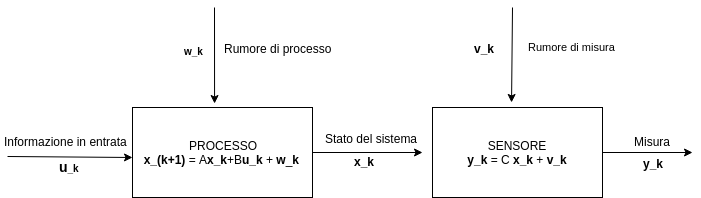
\includegraphics[width=\linewidth]{img/mimo2}
	\caption{Processo e misura caratterizzati da rumore}
	\label{fig:mimo2}
\end{figure}
Dal momento che non \`e possibile individuare una soluzione analitica di $(4)$, il problema da risolvere \`e \emph{stimare} lo stato del sistema $\mathbf{x}_k$ per qualunque istante di tempo $k$.
\subsubsection{Soluzione}
Si definiscono i vettori:
\begin{itemize} 
	\item $\hat{\mathbf{x}}^-_k$ come la stima \emph{a priori} dello stato del sistema all'istante $k$, sulla base della conoscenza del processo all'istante $k-1$;
	\item $\hat{\mathbf{x}}_k$ come la stima \emph{a posteriori} dello stato del sistema all'istante $k$, data dalle misurazioni $\mathbf y_k$ allo stesso istante.
\end{itemize}
Si ha che ciascun $\hat{\mathbf{x}}^-_k$ e ciascun $\hat{\mathbf{x}}_k$ \`e in effetti un vettore di variabili aleatorie.\\*
Siano $\mathbf{e}^-_k = (\mathbf x_ k - \hat{\mathbf{x}}^-_k)$, $\mathbf e_k = (\mathbf x_k - \hat{\mathbf{x}}_k)$ rispettivamente l'\emph{errore} a priori e l'\emph{errore} a posteriori di stima, e siano $P^-_k$ e $P_k$ rispettivamente le matrici di covarianza di $\mathbf{e}^-_k$ e di $\mathbf{e}_k$.\\*
Un KF lineare \`e una quintupla di equazioni:
\begin{enumerate}
\item $
\hat{\mathbf{x}}^-_k = A \hat{\mathbf{x}}^-_{k-1} + B \mathbf u_k
$
\item $ P^-_k = A P^-_{k-1} A^T + Q
$
\item $ L_k = P_k^-C^T(CP_k^-C^T + R)^{-1}
$
\item $ \hat{\mathbf{x}}_k = \hat{\mathbf{x}}^-_k + L_k(\mathbf y_k - C \hat{\mathbf{x}}^-_k)
$
\item $ P_k = (I-L_kC)P^-_k
$
\end{enumerate}
In cui le equazioni $1$ e $2$ vengono dette \emph{equazioni di predizione}. Esse proiettano lo stato del sistema al tempo $k-1$ e la covarianza
dell'errore di stima a priori al tempo $k-1$, in avanti all'istante $k$.\\*
Le equazioni $3$, $4$, $5$, vengono dette \emph{equazioni di aggiornamento}, e costituiscono il modello del meccanismo di \emph{retroazione} con cui il filtro corregge la proprie stime, sulla base delle misurazioni fornite:
\begin{itemize}
	\item Viene prima calcolata $L_k$, ossia la \emph{matrice dei guadagni di Kalman};
	\item Le misure $\mathbf y_k$ vengono usate per determinare una \emph{stima a posteriori} dello stato del sistema all'istante $k$;
	\item Infine viene calcolata una stima della covarianza dell'errore a posteriori $P_k$.
\end{itemize}
In figura \ref{fig:kf}, \`e riportato uno schema del funzionamento logico di un KF collegato a un sistema dinamico lineare a tempo discreto.\\*
\begin{figure}[h]
	\centering
	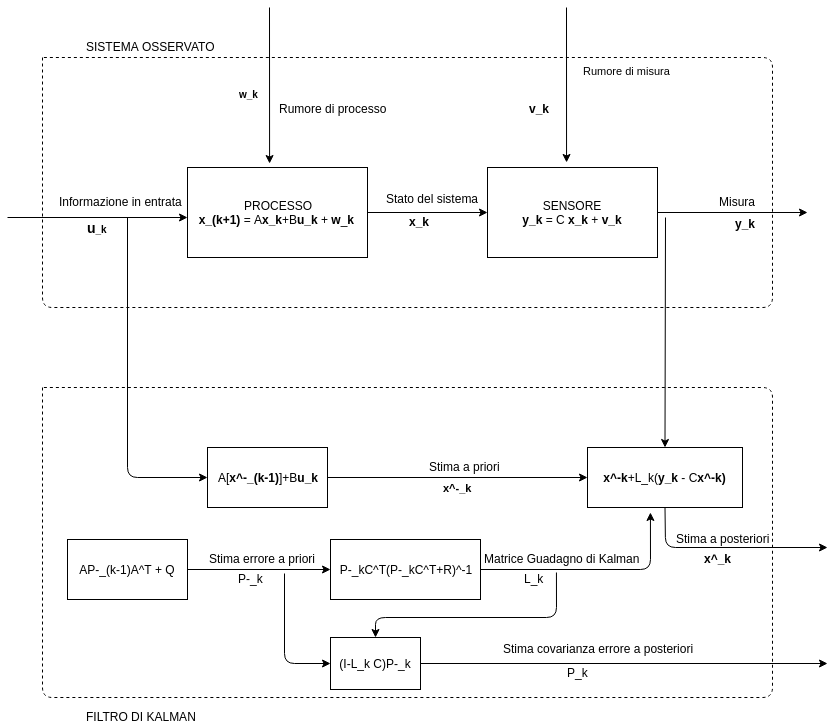
\includegraphics[width=\linewidth]{img/kalman}
	\caption{Schema di un KF lineare}
	\label{fig:kf}
\end{figure}
KF \`e un \emph{filtro ricorsivo}, in quanto la stima $\hat{\mathbf{x}}_k$ dello stato del sistema all'istante $k$ viene determinata combinando le informazioni date dal vettore di misurazioni $\mathbf y_k$ campionate all'istante $k$ con la stima dello stato del sistema all'istante $k-1$\footnote{Supposto noto lo stato iniziale $\mathbf x_0$.}.\\*
KF \`e uno \emph{stimatore ottimo}, dove ottimo significa che minimizza la covarianza dell'errore di stima a posteriori, se tutti i rumori hanno distribuzione normale multivariata. \cite{kfbook}
\newpage
\subsection{Esempio applicativo}
Si supponga di voler stimare i valori di posizione e velocit\`a nel sistema dinamico individuato dalla $(3)$. Valgono le seguenti ipotesi:
\begin{itemize}
	\item Il corpo, modellato come puntiforme, viene lasciato cadere da una quota $z(0) = z_0$ assegnata, con velocit\`a iniziale $v_0$;
	\item La sola accelerazione a cui \`e soggetto il corpo \`e l'accelerazione gravitazionale $-g$;
	\item Il sistema non \`e caratterizzato da rumore di processo;
	\item Un osservatore \`e in grado di misurare la quota dell'oggetto mediante uno strumento di misura $X$ 
	distribuito come una normale univariata con varianza $R$;
	\item Il sistema viene osservato ogni secondo per un intervallo di tempo lungo $t_{M}\;s$.
\end{itemize}
Valori numerici:
\begin{itemize}
	\item $z_0 = 100\;m$
	\item $v_0 = 0 \frac{m}{s}$
	\item $g = 1\;\frac{m}{s^2}$
	\item $R = 1\;m^2$
	\item $t_M = 10\;s$
\end{itemize}
Si scrivono le equazioni $(4)$ modellanti la dinamica del processo evolutivo e la dinamica del processo di misurazione:
$$
\begin{cases}
\mathbf x_k = A \mathbf x_{k-1} + B \mathbf u_k + \mathbf w_k \\
\mathbf y_k = C \mathbf x_k + \mathbf v_k
\end{cases} = 
\begin{cases}
\mathbf x_k = \left(\begin{matrix}
1 & 1 \\
0 & 1 
\end{matrix}\right) \mathbf x_{k-1} + \left(\begin{matrix}
\frac{1}{2} \\
1
\end{matrix}\right) -g + \underline 0 \\
\mathbf y_k = \left(\begin{matrix}
1\\
0
\end{matrix}\right) \mathbf x_k + \mathbf v_k
\end{cases} = 
$$
$$
= \begin{cases}
\mathbf x_k = \left(\begin{matrix}
1 & 1 \\
0 & 1 
\end{matrix}\right) \mathbf x_{k-1} - \left(\begin{matrix}
\frac{1}{2} \\
1
\end{matrix}\right) \\
\mathbf y_k = \left(\begin{matrix}
1\\
0
\end{matrix}\right) \mathbf x_k + \mathbf v_k
\end{cases}
$$
Il Filtro di Kalman \`e dato dalle seguenti equazioni:
\begin{itemize}
	\item \begin{enumerate}
		\item[$1.$] $
		\hat{\mathbf{x}}^-_k = A \hat{\mathbf{x}}^-_{k-1} + B \mathbf u_k =$\\*
		$= \left(\begin{matrix}
		1 & 1 \\
		0 & 1 
		\end{matrix}\right) \hat{\mathbf{x}}^-_{k-1} - \left( \begin{matrix}
		\frac{1}{2}\\
		1
		\end{matrix}\right)
		$
		\item[$2.$]  $ P^-_k = A P^-_{k-1} A^T + Q =$\footnote{Non essendoci rumore di processo, la matrice $Q$ di covarianza di tale quantit\`a \`e la matrice nulla.}\\*
		$= \left(\begin{matrix}
		1 & 1 \\
		0 & 1 
		\end{matrix}\right) P^-_{k-1}\left(\begin{matrix}
		1 & 1 \\
		0 & 1 
		\end{matrix}\right)^T + 0$        
	\end{enumerate}
	\item
	\begin{enumerate}
		\item[$3.$] $ L_k = P_k^-C^T(CP_k^-C^T + R)^{-1}
		 = $\\*
		 $ = P_k^-\left(\begin{matrix}
		 1\\
		 0
		 \end{matrix}\right)^T \left[ \left(\begin{matrix}
		 1\\
		 0
		 \end{matrix}\right)P_k^-\left(\begin{matrix}
		 1\\
		 0
		 \end{matrix}\right)^T + 1
		 \right]^{-1} =
		 $
		\item[$4.$] $ \hat{\mathbf{x}}_k = \hat{\mathbf{x}}^-_k + L_k(\mathbf y_k - C \hat{\mathbf{x}}^-_k) =
		$\\*
		$
		= \hat{\mathbf{x}}^-_k + L_k\left[ \mathbf y_k - \left(\begin{matrix}
		1\\
		0
		\end{matrix}\right) \hat{\mathbf{x}}^-_k\right]
		$
		\item[$5.$] $ P_k = (I-L_kC)P^-_k =
		$
		\\*
		$
		= \left[ \left(\begin{matrix}
		1 & 0\\
		0 & 1
		\end{matrix}\right)-L_k\left(\begin{matrix}
		1\\
		0
		\end{matrix}\right)\right]P^-_k
		$
	\end{enumerate}
\end{itemize}
Assegnato lo stato iniziale:
$$
\mathbf x_0 = (z_0,v_0) = (100, 0)
$$
Si ha che la stima a priori dello stato del sistema all'istante $0$ vale esattamente lo stato iniziale noto del sistema:
$$
\hat{\mathbf{x}}^-_{0} = \mathbf x_0 = (z_0,v_0) = (100,0)
$$
Mentre la matrice di covarianza dell'errore a priori viene inizializzata come la matrice di covarianza della sorgente delle misurazioni:
$$
P^-_{0} = R = 1
$$
Supponendo di effettuare, attraverso lo strumento $X$, le misure riportate in tabella \ref{tab:misurekalman}, un esempio di implementazione in linguaggio MATLAB\footnote{Le motivazioni della scelta di MATLAB sono da ricercarsi nella natura del linguaggio: esso \`e fortemente orientato al calcolo numerico e alla manipolazione efficiente di espressioni matriciali.} del KF descritto \`e mostrato di seguito.
\begin{table}[h]
	\centering
	\begin{tabular}{|c|c|c|c|c|c|c|c|c|c|c|}
		\hline 
		$\mathbf{t\;(s)}$ & $1$ & $2$ & $3$ & $4$ & $5$ & $6$ & $7$ & $8$ & $9$ & $10$ \\ 
		\hline 
		$\mathbf{y_t\;(m)}$ & $100$ & $97.9$ & $94.9$ & $92.7$ & $87.3$ & $81.3$ & $75.8$ & $67.5$ & $59.17$ &$51.1$ \\ 
		\hline 
	\end{tabular} 
	\caption{Misurazioni di esempio del corpo in caduta libera}
	\label{tab:misurekalman}
\end{table}
\subsubsection{Codice Soluzione}
Si riporta in questa sezione il codice risolutivo del problema individuato.
\lstinputlisting[language=MATLAB, firstline=1, lastline=7, caption ={Definizione delle variabili del problema}]{Models/kalmanexample.m}

\lstinputlisting[language=MATLAB, firstline=11, lastline=20, caption ={Inizializzazione del Filtro di Kalman}]{Models/kalmanexample.m}
\newpage
\lstinputlisting[language=MATLAB, firstline=22, lastline=38, caption ={Algoritmo individuato dalle Equazioni di KF}]{Models/kalmanexample.m}
\newpage
\subsubsection{Risultati}
Nelle figure \ref{fig:predspeed}, \ref{fig:predheight} viene mostrato il grafico che compara i valori stimati di velocit\`a e posizione con i veri valori delle medesime grandezze; infatti tali valori sono determinabili analiticamente come soluzioni esplicite della $(3)$.\\*
Tali grafici danno un'idea immediata della capacit\`a che ha l'algoritmo di stimare la posizione e la velocit\`a in maniera affidabile anche in presenza di un processo di misura affetto da rumore.\\*
\begin{figure}[h]
	\centering
	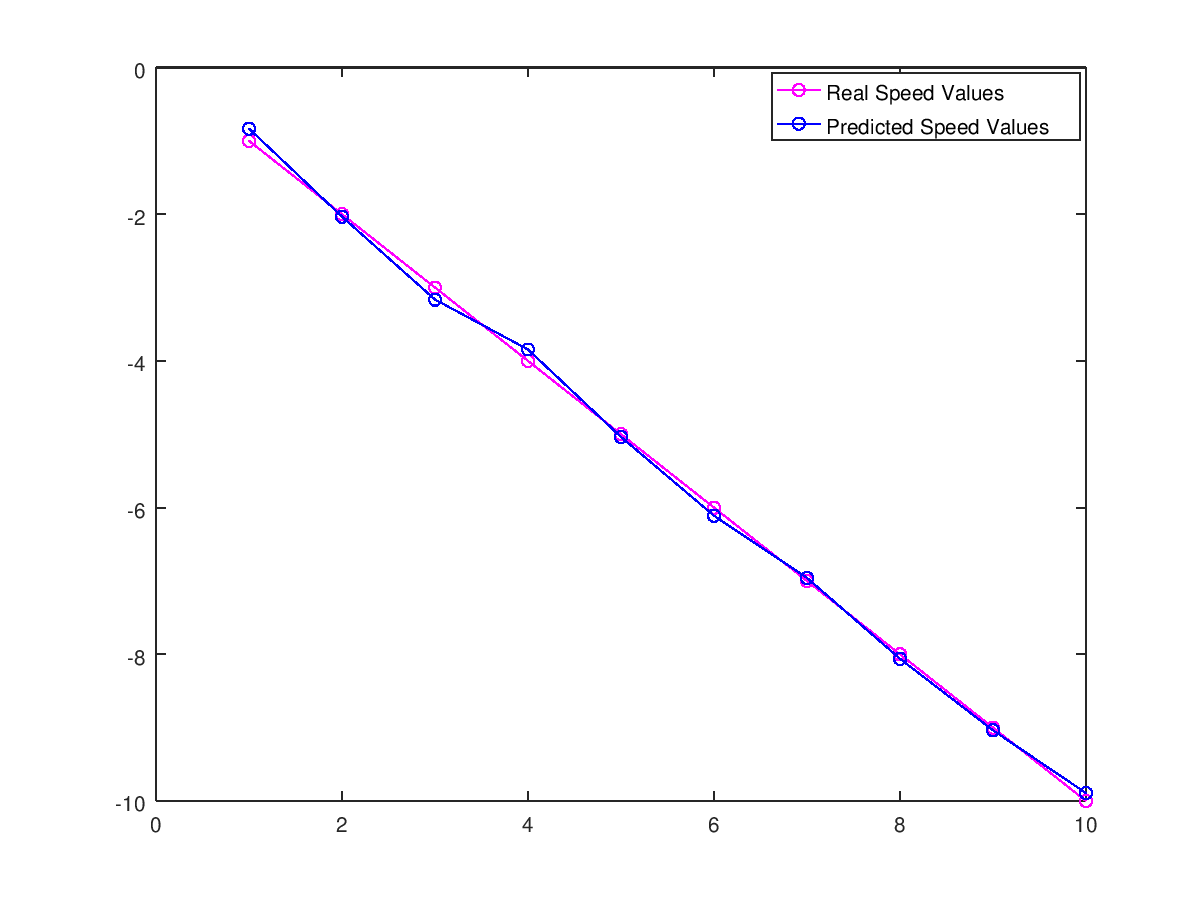
\includegraphics[scale=0.7]{img/predspeed}
	\caption{Stima della velocit\`a del corpo in caduta}
	\label{fig:predspeed}
\end{figure}
\begin{figure}[h]
	\centering
	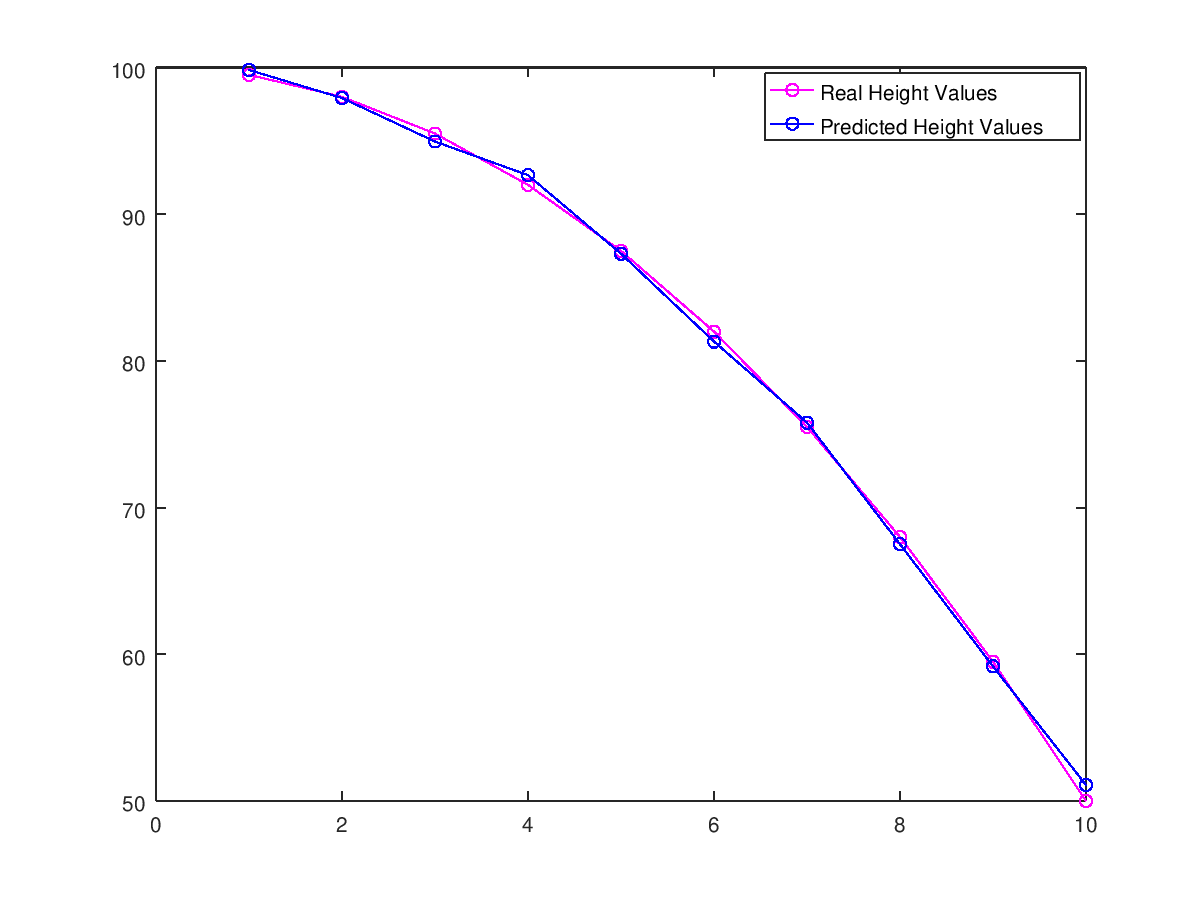
\includegraphics[scale=0.7]{img/predheight}
	\caption{Stima della posizione del corpo in caduta}
	\label{fig:predheight}
\end{figure}
\newpage
In tabella \ref{tab:syntex} viene riportata una sintesi dei dati prodotti dall'esecuzione dell'algoritmo.\\*
\begin{table}[h]
	\begin{tabular}{|c|c|c|c|c|c|}
		\hline 
		$\mathbf{t}\;(s)$ & \textbf{Misura (m)} & \textbf{Pos.(m)} & \textbf{Stima Pos. (m)} & \textbf{Vel.} $\mathbf{\left(\frac{m}{s}\right)}$ & \textbf{Stima Vel.} $\mathbf{\left(\frac{m}{s}\right)}$ \\ 
		\hline 
		$1$ & $100$ & $99.5$ & $99.833$ & $-1$ & $-0.83333$ \\ 
		\hline 
		$2$ & $97.9$ & $98$ & $97.9167$ & $-2$ & $-2.0333$ \\ 
		\hline 
		$3$ & $94.9$ & $95.5$ & $94.9545$ & $-3$ & $-3.1636$ \\ 
		\hline 
		$4$ & $92.7$ & $92$ & $92.6611$ & $-4$ & $-3.8444$ \\ 
		\hline 
		$5$ & $83.7$ & $87.5$ & $87.3074$ & $-5$ & $-5.037$ \\ 
		\hline 
		$6$ & $81.3$ & $82$ & $81.3184$ & $-6$ & $-6.1105$ \\ 
		\hline 
		$7$ & $75.8$ & $75.5$ & $75.7941$ & $-7$ & $-6.9588$ \\ 
		\hline 
		$8$ & $67.5$ & $68$ & $67.5076$ & $-8$ & $-8.0606$ \\ 
		\hline 
		$9$ & $59.17$ & $59.5$ & $59.174$ & $-9$ & $-9.0358$ \\ 
		\hline 
		$10$ & $51.1$ & $50$ & $51.0892$ & $-10$ & $-9.8922$ \\ 
		\hline 
	\end{tabular} 
	\caption{Risultati generali dell'algoritmo}
	\label{tab:syntex}
\end{table}
Nelle tabelle \ref{tab:errors} e \ref{tab:errorsmeas} \`e mostrato un paragone fra l'errore a posteriori $(\mathbf x_k - \mathbf{\tilde{x}}_k)$ e l'errore della misura rispetto alla posizione reale.\\*
Si noti che per ciascun istante $t$, l'errore a posteriori sul valore di posizione \`e minore, in valore assoluto, della distanza fra la misura osservata e la posizione reale del corpo.\\*
Questo porta alla conclusione che l'utilizzo di KF ha permesso di ottenere misure sempre pi\`u affidabili rispetto a quelle ottenute dalla sorgente.
\begin{table}[h]
	\begin{tabular}{|c|c|c|c|}
		\hline 
		$\mathbf{t}\;(s)$ & $\mathbf{\hat{x}}_k$ & $\mathbf x_k$ & $\mathbf x_k - \mathbf{\hat{x}}_k$ \\ 
		\hline 
		$1$&$(99.833,-0.83333)$&$(99.5,-1)$  & $(-0.333333,-0.166667)$
		   \\ 
		\hline 
		$2$&$(97.9167,-2.0333)$ & $(98,-2)$ & $(0.083333,0.033333)$
		
		   \\ 
		\hline 
		$3$& $(94.9545,-3.1636)$ & $(95.5,-3)$ & $(0.545455,0.163636)$
		
		  \\ 
		\hline 
		$4$&  $(92.6611,-3.8444)$ & $(92,-4)$ &$(-0.661111,-0.155556)$
		
		  \\ 
		\hline 
		$5$&$(87.3074,-5.037)$  & $(87.5,-5)$ &  $(0.192593,0.037037)$
		  \\ 
		\hline 
		$6$& $(81.3184,-6.1105)$ & $(82,-6)$ &  $(0.681579,0.110526)$
		  \\ 
		\hline 
		$7$&  $(75.7941,-6.9588)$ & $(75.5,-7)$ &  $(-0.294118,-0.041176)$
		  \\ 
		\hline 
		$8$& $(67.5076,-8.0606)$ & $(68,-8)$ &  $(0.492424,0.060606)$
		  \\ 
		\hline 
		$9$&  $(59.174,-9.0358)$ & $(59.5,-9)$ &  $(0.326024,0.035783)$
		  \\ 
		\hline 
		$10$& $(51.0892,-9.8922)$ & $(50,-10)$ & $(-1.089216,-0.107843)$
		  \\ 
		\hline 
	\end{tabular} 
	\caption{Errori a posteriori}
	\label{tab:errors}
\end{table}
\begin{table}[h]
	\begin{tabular}{|c|l|r|}
		\hline 
		$\mathbf{t}\;(s)$ & \textbf{Errore a posteriori (pos.) (m)} & $\Delta \mathbf{(pos,misura)}$ \textbf{(m)} \\ 
		\hline 
		$1$ & $-0.333333$ & $(99.500 - 100) =-0.5$ \\ 
		\hline 
		$2$ & $0.083333$ & $(98 - 97.9) = 0.1$ \\ 
		\hline 
		$3$ & $0.545455$ & $(95.5-94.9) = 0.6$ \\ 
		\hline 
		$4$ & $-0.661111$ & $(92 - 92.7) = -0.7$ \\ 
		\hline 
		$5$ &  $0.192593$ & $(87.5 - 87.3) = 0.2$ \\ 
		\hline 
		$6$ & $0.681579$ & $(82 - 81.3) = 0.7$ \\ 
		\hline 
		$7$ & $-0.294118$ & $(75.5 - 75.8) = -0.3$ \\ 
		\hline 
		$8$ & $0.492424$ & $(68 - 67.5) = 0.5$ \\ 
		\hline 
		$9$ & $0.326024$ & $(59.5 - 59.17) = 0.33$ \\ 
		\hline 
		$10$ & $-1.089216$ & $(50-51.1) = -1.1$ \\ 
		\hline 
	\end{tabular} 
	\caption{Confronto tra errore a posteriori sulla posizione, e distanza fra valori reali di posizione e misure di posizione}
	\label{tab:errorsmeas}
\end{table}
\clearpage
\subsection{Filtri di Kalman non Lineari}
I fenomeni reali sono raramente lineari. Un modello lineare \`e spesso un'approssimazione di un modello pi\`u complesso. \cite{gigi}\\*
Nel dominio applicativo in cui si colloca la Tesi, ossia quello del posizionamento ferroviario, occorre utilizzare una generalizzazione al caso non-lineare dei KF standard.\\*
Si pu\`o modellare un sistema dinamico discreto non lineare, caratterizzato da rumore, come:
$$
\begin{cases}
\mathbf{x}_k = F(\mathbf{x}_k,\mathbf{w}_k) \\
\mathbf{y}_k = H(\mathbf{x}_k,\mathbf{v}_k)
\end{cases}
$$
In cui, in analogia con il caso lineare:
\begin{itemize}
	\item $\mathbf x_k$ rappresenta lo stato del sistema all'istante $k$
	\item $\mathbf w_k$ rappresenta il rumore di processo all'istante $k$
	\item $\mathbf y_k$ rappresenta il vettore di misurazioni campionate all'istante $k$
	\item $\mathbf v_k$ rappresenta il rumore di misura all'istante $k$
\end{itemize}
A differenza del modello lineare, le funzioni $F,H$ che descrivono le dinamiche del processo evolutivo e del processo di misura, non sono in generale lineari. \cite{ukffne}\\*
Esistono diverse forme di KF non lineari, nel seguito della Tesi l'implementazione di SFA cui verr\`a fatto riferimento, \`e basata sull'utilizzo di un \emph{Unscented Kalman Filter} (UKF).